\documentclass{article} % \documentclass{} is the first command in any LaTeX code.  It is used to define what kind of document you are creating such as an article or a book, and begins the document preamble

\usepackage{amsmath} % \usepackage is a command that allows you to add functionality to your LaTeX code
\usepackage{graphicx}
\graphicspath{ {./images/} }
\title{Discrete Time Signals and Systems} % Sets article title
\author{Hunter Mills} % Sets authors name
\date{\today} % Sets date for date compiled

% The preamble ends with the command \begin{document}
\begin{document} % All begin commands must be paired with an end command somewhere
    \maketitle % creates title using information in preamble (title, author, date)
    
    \section{Frequency Analysis of Signals} % creates a section
    Two of the most important mathematical tools in engineering is the Fourier Transform and Fourier Series. In this chapter they will be used to do frequency analysis. This signal representations basically involve the decomposition of the signals into terms of sinusoidal functions. For infinite periodic signals, use the Fourier series and for a finite energy series use the Fourier transform. These decomposition are very important in LTI systems since the response of an LTI signal to a sinusoid is a sinusoid of the same frequency but different amplitude and phase.
    \subsection{Euler's Identity}
    \begin{equation}
 	e^{j\theta} = \cos(\theta) + j\sin(\theta)
	\end{equation}
	\begin{equation}
 	\cos(\theta) = \frac{e^{j\theta} + e^{-j\theta}}{2}
	\end{equation}
	\begin{equation}
 	\sin(\theta) = \frac{e^{j\theta} - e^{-j\theta}}{j2}
	\end{equation}
	\begin{equation}
 	\cos(\Omega_k t) = \frac{1}{2}(e^{j\Omega_k t} + e^{-j\Omega_k t})
	\end{equation}
	\begin{equation}
 	\sin(\Omega_k t) = \frac{-j}{2}(e^{j\Omega_k t} - e^{-j\Omega_k t})
	\end{equation}
    
    \subsection{Frequency Analysis of Continuous Time Signals}
    \textbf{The Fourier Series for CT Periodic Signals}
    
    The Fourier Series is a representation of the signal as a linear weighted sum of harmonically related sinusiods or complex exponentials. From chapter 1, we can recall that a linear combination of harmonically related complex exponentials of the form
    \begin{equation}
 	x(t) = \sum_{k=-\infty}^{\infty}c_ke^{j2\pi kF_0t}     
	\end{equation}
	is a periodic signal with fundamental period $T_P = 1/F_0$. Hence we can think of the exponential signals
	\begin{equation}
 	 {e^{j2\pi kF_0t}, \;\;\;\;\;\; k = 0, \pm 1, \pm 2 ...}
	\end{equation}
	as the building blocks to construct periodic signals by the proper choice of fundamental frequency and $c_k$. The Fourier series coefficients can be calculated with:
	\begin{equation}
 	c_k = \frac{1}{T_P} \int_{T_P} x(t)e^{-j2 \pi kF_0t}dt.
	\end{equation}
	In general the Fourier coefficients $c_k$ are complex. It is easily shown that if the periodic signal is real, $c_k$ and $c_{-k}$ are complex conjugates. As a result:
	\begin{equation}
 	c_k = |c_k|e^{j\theta_{k}}
	\end{equation}
	then
	\begin{equation}
 	c_{-k} = |c_k|^{-j\theta_{k}}
	\end{equation}
	Consequently the FS can be represented as:
	\begin{equation}
 	x(t) = c_0 + 2\sum_{k=1}^{\infty}|c_k|\cos(2\pi k F_0t + \theta_{k})    
	\end{equation}
	or 
	\begin{equation}
 	Trigonometric: x(t) = a_0 + \sum_{k=1}^{\infty}(a_k\cos(2\pi kF_0t) - b_k\sin(2\pi kF_0t))
	\end{equation}
	\begin{equation}
 	Harmonic: x(t) = A_{DC} + \sum_{k=1}^{\infty}\sqrt{a_k^2+b_k^2} \cos(\Omega_{k}t - \theta_{k}) 
	\end{equation}
	where $a_0 = c_0$, $a_k = 2|c_k|\cos(\theta_{k})$, and $b_k = 2|c_k|\sin(\theta_{k})$\\
	\\
	\textbf{Power Density Spectrum of Periodic Signals}\\
	
	A periodic signal has infinite energy and a fine average power. Using the FS the \textbf{Parsevals Relation for Power Signals} becomes clear.
	\begin{equation}
 	P_x = \frac{1}{T_P} \int_{T_P} |x(t)|^2dt = \sum_{k=-\infty}^{\infty} |c_k|^2
	\end{equation}
	If we would plot $|c_k|^2$ as a function of the frequencies $kF_0, k=0,\pm 1, \pm 2,...$ then figure 1 shows the \textit{power density spectrum}.
	
	\begin{figure}[h]
    \centering
	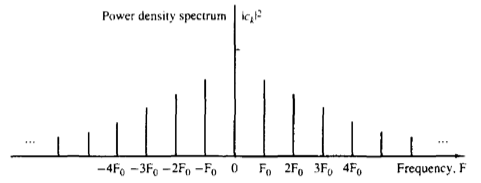
\includegraphics[width=10cm]{pds}
	\caption{Power Density Spectrum}
	\end{figure}
	
	This is called a line spectrum and the spacing between the spectral lines is the fundamental frequency. The total average power can be expressed as 
	\begin{equation}
 	P_x = c_0^2 + 2\sum_{k=1}^{\infty}|c_k|^2
	\end{equation}
	\begin{equation}
 	P_x = a_0^2 + \frac{1}{2}\sum_{k=1}^{\infty}(a_k^2 + b_k^2)
	\end{equation}
	\\
	\\
	\textbf{•}

	
\end{document} % This is the end of the document